% https://tex.stackexchange.com/a/390396/173708
\documentclass[12pt,a4paper]{standalone}
\usepackage[utf8]{inputenc}
\usepackage{graphicx,tikz}

\begin{document}
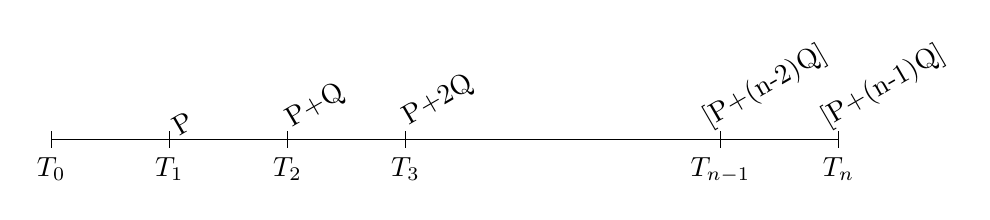
\begin{tikzpicture}[scale=1,rotLabel/.style={above,rotate=30,anchor=200}]
 % draw horizontal line 
  \draw (0,0) -- (10,0);
  % draw vertical lines
   \foreach \x in {0,1.5,3,4.5,8.5,10}
   \draw (\x cm,3pt) -- (\x cm,-3pt);
    % draw nodes
   \draw (0,0) node[below=3pt] {$T_0$ } node[rotLabel] {};
   \draw (1.5,0) node[below=3pt] {$T_1$} node[rotLabel] {P};
   \draw (3,0) node[below=3pt] {$T_2$} node[rotLabel] {P+Q};
   \draw (4.5,0) node[below=3pt] {$T_3$} node[rotLabel] {P+2Q};
   \draw (8.5,0) node[below=3pt] {$T_{n-1}$} node[rotLabel] {[P+(n-2)Q]};
   \draw (10,0) node[below=3pt] {$T_n$} node[rotLabel] {[P+(n-1)Q]};
   \end{tikzpicture}
\end{document}